\chapter{Análisis} \label{analisis}
\epigraph{\textit{Research is what I'm doing when I don't know what I'm doing.   
	}}{\textit{— Wernher von Braun, NASA engineer}}
	\vspace*{8cm}
	\begin{center}
		\centering
		\includegraphics[width=10.5cm]{example-image}
    \end{center}
\thispagestyle{empty}
\newpage
\vspace*{2cm}

\section{Estudio de factibilidad}
En esta sección del trabajo terminal, abordaremos la factibilidad técnica y económica que tendrá la implementación de la solución propuesta. Para ello se dará respuesta a las siguientes preguntas sobre la factibilidad del sistema.

\textbf{\textit{¿Este sistema implementará alguna tecnología que no se haya empleado previamente?}}\newline
Para el desarrollo del sistema no requerirá alguna tecnología que no se haya implementado anteriormente, ya que los usuarios deberán contar con un dispositivo móvil para realizar las actividades necesarias para el funcionamiento de este. 

\textbf{\textit{¿El sistema puede integrarse dentro de alguna organización?}}\newline
El sistema se plantea como un sistema independiente, pero, puede hacerlo adaptando el sistema para que sea consumido por otros que estén en la organización que lo use.

\textbf{\textit{Considerando gastos, tecnología, conocimiento y tiempo ¿El desarrollo del sistema es conveniente?}}\newline
La respuesta es sí, ya que la tecnología que implementará tiene una gran comunidad y tiene años en el mercado, lo único necesario es acceso a un equipo de computo y tener acceso a internet, con lo que ya se cuenta. Los problemas son la falta de conocimiento técnico con algunos temas, sin embargo, el tiempo y apoyándose con la comunidad de desarrolladores que tiene las tecnologías a usar, se puede superar este problema, por otro lado puede que algunas tecnologías tengan algún costo, pero como se tiene acceso a una cuenta universitaria, existen descuentos o inclusive el uso gratuito de la tecnología que se requiera.

Por lo tanto, podemos concluir que el sistema es factible de manera técnica y económicamente.
\subsection{Herramientas necesarias para el desarrollo del sistema}

\subsection{Elección de software}

\section{Metodología}
Para este trabajo terminal se utilizará la metodología de desarrollo rápido de aplicaciones (DRA), dado que el tiempo de desarrollo es corto, esta metodología permite centrarse en el producto final, hace hincapié en el desarrollo de prioridades y la definición de los plazos de entrega, si estos empiezan a atrasarse permite la reducción de requisitos para el ajuste y de esta manera no aumentar la fecha limite de entrega. Por otro lado la participación de los usuarios es necesaria para el diseño del sistema.\cite{dra}

\begin{figure}[!ht]
    \centering
    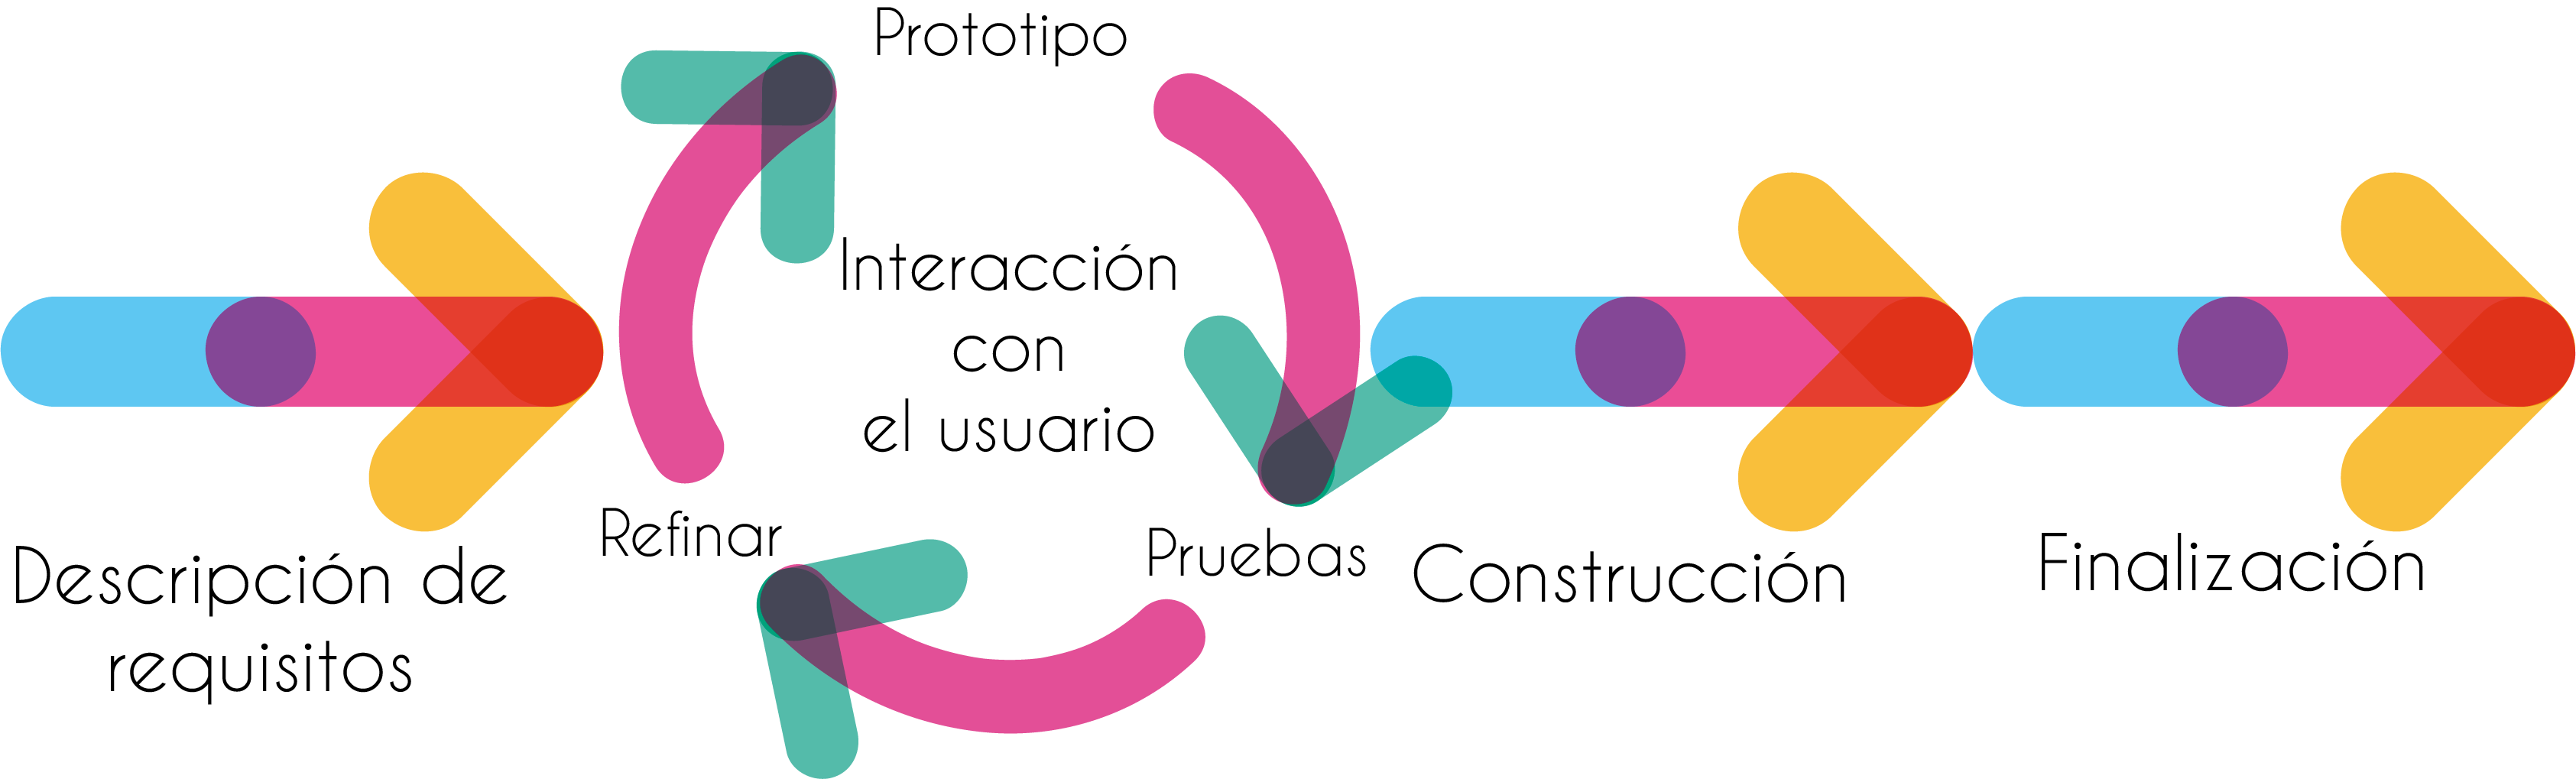
\includegraphics[scale=0.50]{TT/img/metodología/RAD.png}
    \caption{Desarrollo rápido de aplicaciones}
    \label{graphic:RAD}
\end{figure}
\section{Requerimientos}

\subsection{Requerimientos funcionales}

\subsection{Requerimientos no funcionales}

